\documentclass{article}

% Language setting
% Replace `english' with e.g. `spanish' to change the document language
\usepackage[english]{babel}

% Set page size and margins
% Replace `letterpaper' with `a4paper' for UK/EU standard size
\usepackage[letterpaper,top=2cm,bottom=2cm,left=3cm,right=3cm,marginparwidth=1.75cm]{geometry}

% Useful packages
\usepackage{svg}
\svgsetup{inkscapelatex=false}
\usepackage{amsmath}
\usepackage{graphicx}
\usepackage[colorlinks=true, allcolors=blue]{hyperref}
\usepackage{subfigure}

\newcommand{\todo}[1]{{\sf[{\footnotesize{{\color{blue} To Do: #1}}]}}}

\title{TDT4265 Computer Vision and Deep Learning - Final Project}
\author{Project group 102: Marco Kugler, Pia Bauspieß}

\begin{document}
\maketitle
\section*{Task 1: Dataset exploration}

The original dataset consists of 1,905 LIDAR-images (1604 for traning, 301 for validation) collected in traffic in the area around NTNU campus Gløshaugen in Trondheim, Norway. The updated version with additional images annotated by our fellow classmates and ourselves consists of a total of 16,997 images (16,696 for training, 301 for validation). Each image is comprised of three 360° LIDAR-channels with a resolution of 128 pixels in height and 1,024 pixels in width. Within the dataset, moving objects in traffic out of the following eight object categories are annotated: car, truck, bus, motorcycle, bicycle, scooter, person, and rider. All other objects are are attributed to the background class.

For a first overview of the dataset, we visualised all images in randomly selected batches of 80 images for both the training data set, the updated traning dataset, and the validation set. In the first step, the three LIDAR channels are interpreted as RGB images as proposed in the task description. Subsequently, we investigated each image channel individually, as well as images that contain at least one object of a chosen category. An overview of this initial exploration for the original training dataset is given in Figure \ref{fig:overview}\footnote{Figure \ref{fig:overview} is merely supposed to show the methodology of our exploration, not the content of single images, which are therefore printed only at a small scale in this document.}, while the entire visualisation of the original training set, the updated training set, and the validation set can be accessed at \textcolor{red}{insert Google drive link to data exploration}.

\begin{figure}[h!]
    \centering
    \subfigure[]{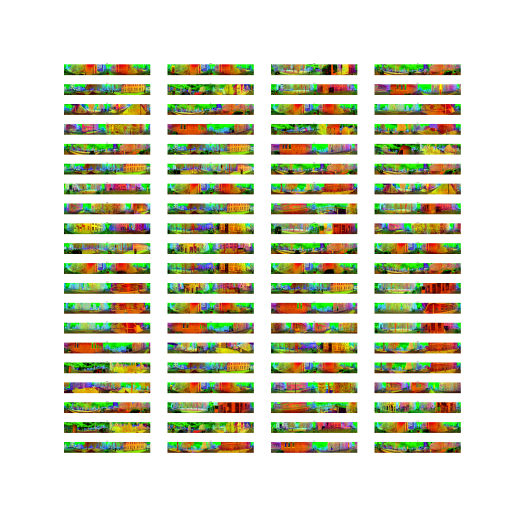
\includegraphics[width=0.16\textwidth]{image_overview/random_all_channels_train_small.png}} 
    \subfigure[]{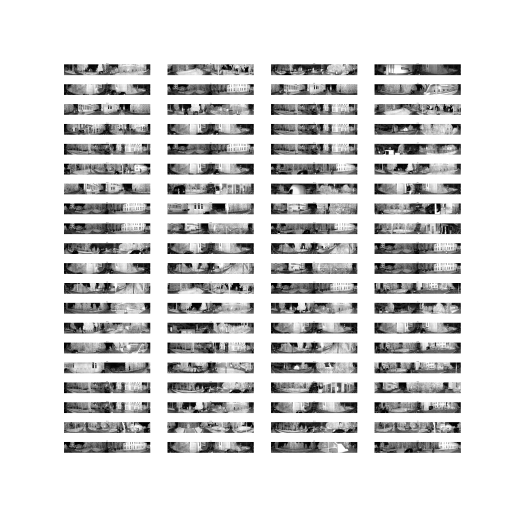
\includegraphics[width=0.16\textwidth]{image_overview/random_channel1_train_small.png}} 
    \subfigure[]{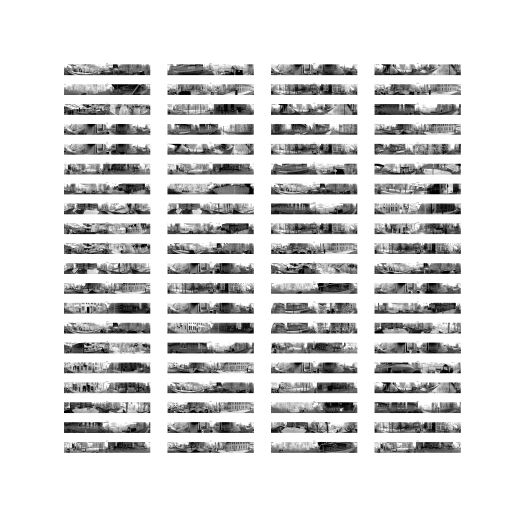
\includegraphics[width=0.16\textwidth]{image_overview/random_channel2_train_small.png}}
    \subfigure[]{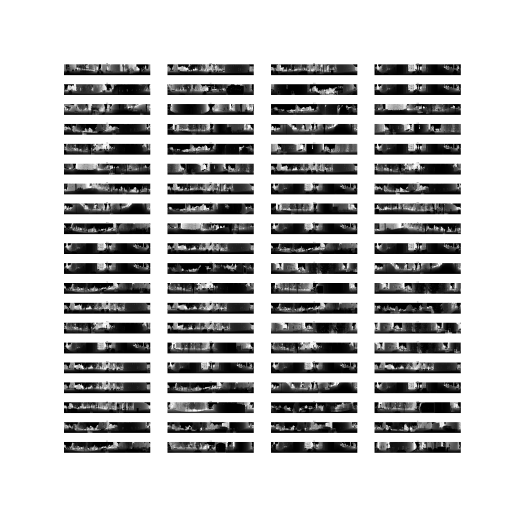
\includegraphics[width=0.16\textwidth]{image_overview/random_channel3_train_small.png}}
    \subfigure[]{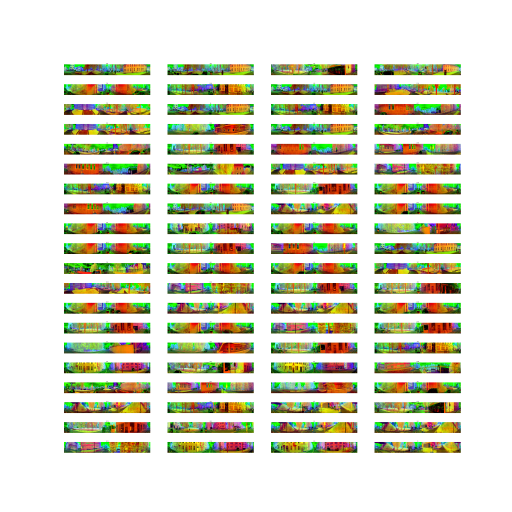
\includegraphics[width=0.16\textwidth]{image_overview/random_car(1)_train_small.png}}
    \subfigure[]{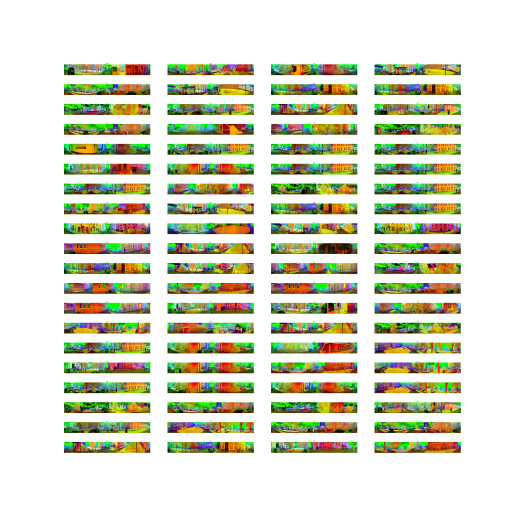
\includegraphics[width=0.16\textwidth]{image_overview/random_person(7)_train_small.png}}
    \caption{Randomly selected images from the original training set showing (a) all three channels combined (b) the first channel (depth) (c) the second channel (ambience) (d) the third channel (intensity) (e) cars (f) persons.}
    \label{fig:overview}
\end{figure}

\subsubsection*{Quantitative analysis}
The prevalent object class in the original training set are cars (52.3\%), followed by persons (26.8\%) and riders of vehicles (8.7\%). This can be seen both from Figure \ref{fig:ratio}, which shows the ratio of labels over the original training set, the updated training set, and the validation set, as well as Figure \ref{fig:occurrence} (a), showing the total occurrence of labels in the training set, the updated training set, and the validation set. While this observation is roughly consistent with the updated extended training set (51.9\% cars, 32.3\% persons, 4.9\% bicycles), the distribution differs significantly from the validation set. Here, the most prevalent object class are persons (66.7\%), followed by cars (25.9\%) and riders (5.7\%). Notably, the validation set does not contain any images with trucks, bicycles, scooters or motorcycles. The existence of riders in the absence of any vehicles that transport riders (bicycles, scooters and motorcycles) in the validation set raises questions, which will be discussed in the following.

Figure \ref{fig:occurrence} offers more insight into correlations of annotated objects, where plot (b) illustrates the occurrence of objects only in images where the label is present, excluding images that do not contain an object of a chosen class. Thereby, grouped occurrences of labels can be detected. For instance, such groupings become visible for bicycles and scooters, but not so much for cars and persons. In other words, if there is a bicycle in an image, it is likely that there are more bicycles in the same image. For persons, Figure \ref{fig:occurrence} indicates that almost all images contain persons, as the value barely fluctuates from subplot \ref{fig:occurrence} (a) to subplot \ref{fig:occurrence} (b).

\begin{figure}[t]
    \centering
    \subfigure[]{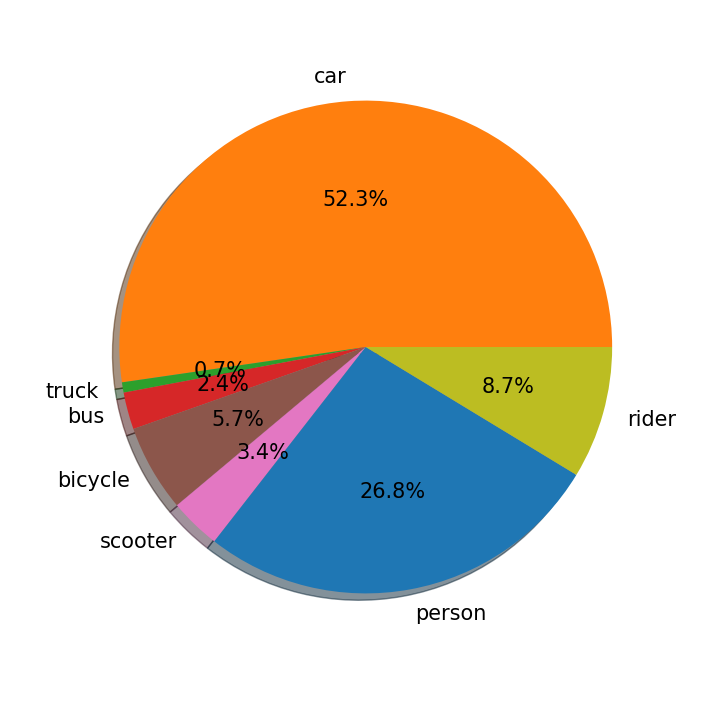
\includegraphics[width=0.32\textwidth]{label_distribution/train/label_ratio_train_cropped.png}}
    \subfigure[]{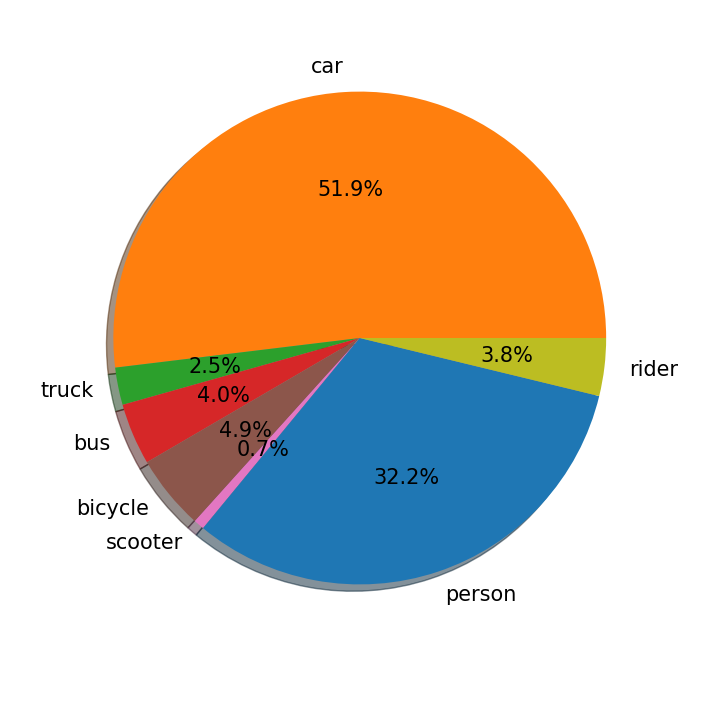
\includegraphics[width=0.32\textwidth]{label_distribution/extended_train/label_ratio_extended_train.png}} 
    \subfigure[]{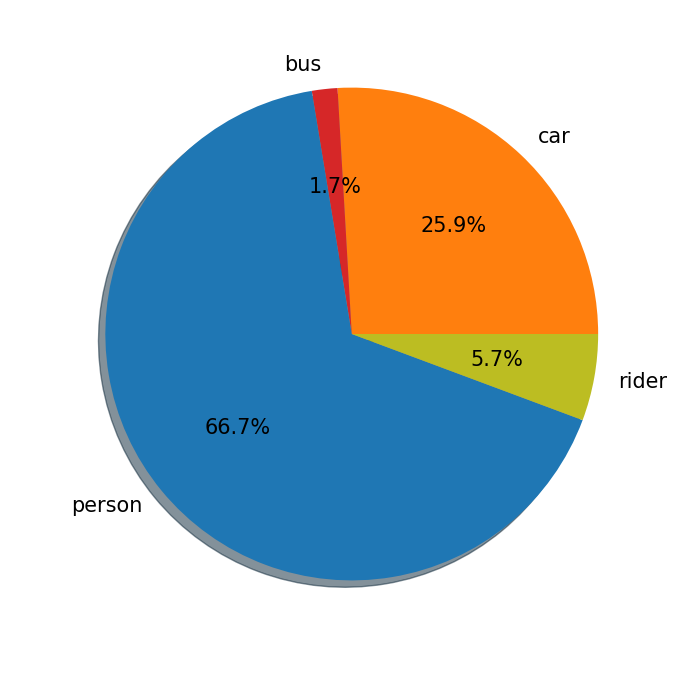
\includegraphics[width=0.32\textwidth]{label_distribution/val/label_ratio_val_cropped.png}} 
    \caption{Label ratios over (a) original training set (b) updated training set (c) validation set.}
    \label{fig:ratio}
\end{figure}

\begin{figure}[t!]
    \centering
    %\subfigure[]{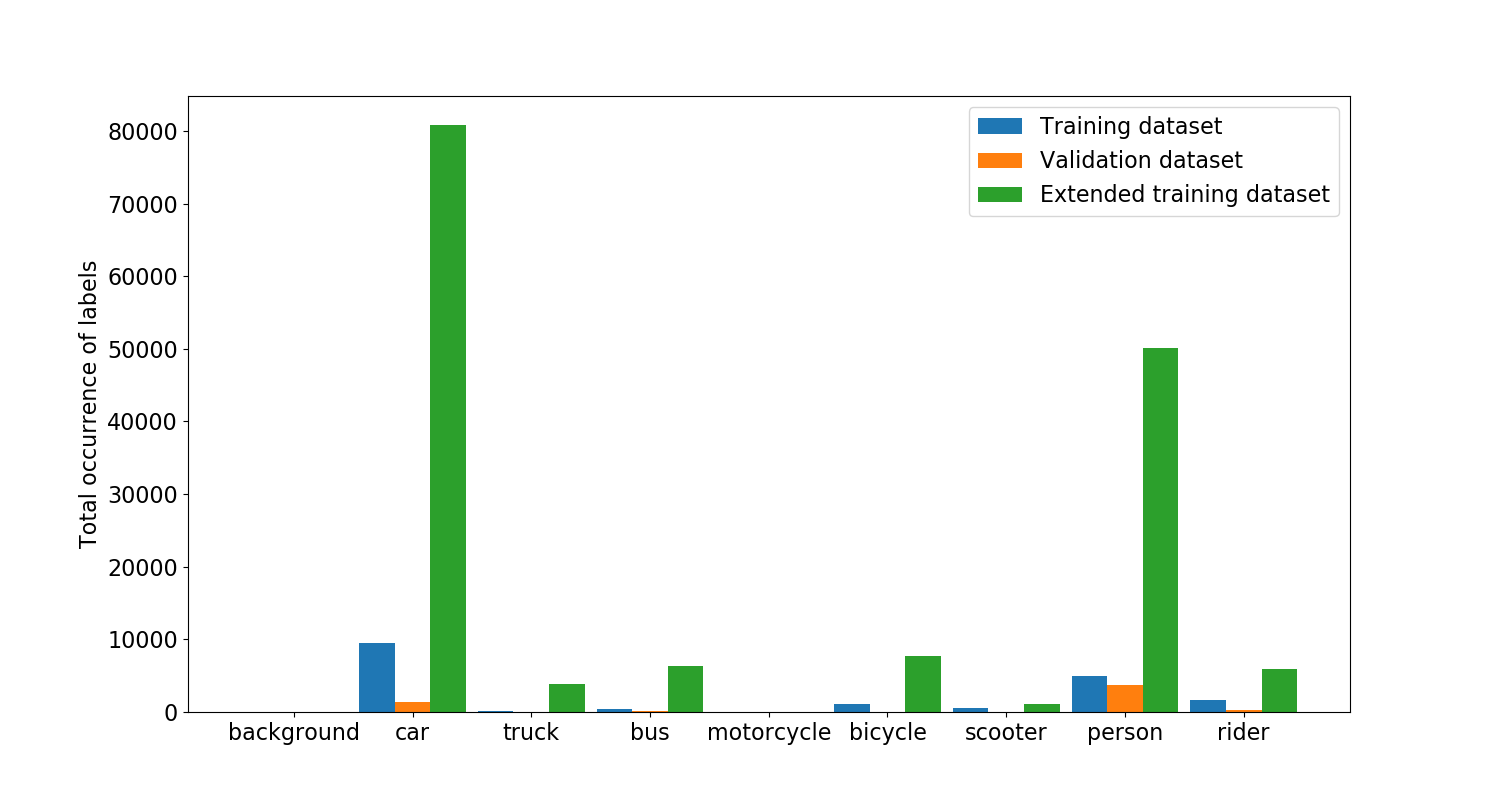
\includegraphics[width=0.49\textwidth]{label_distribution/comparison/total_occurence_comparison.png}}
    %\subfigure[]{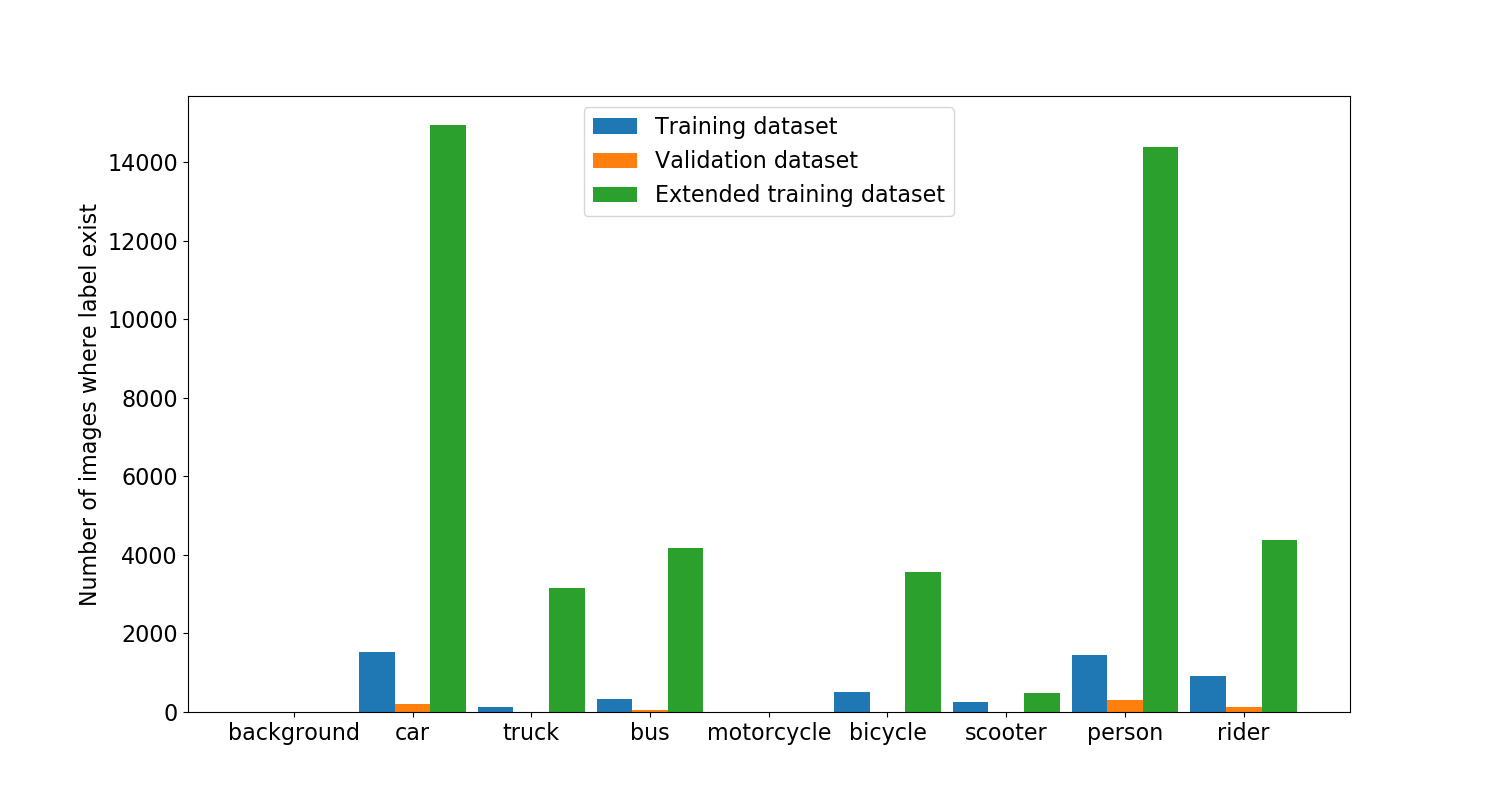
\includegraphics[width=0.49\textwidth]{label_distribution/comparison/number_images_where_label_exist_comparison.png}} 
    \subfigure[]{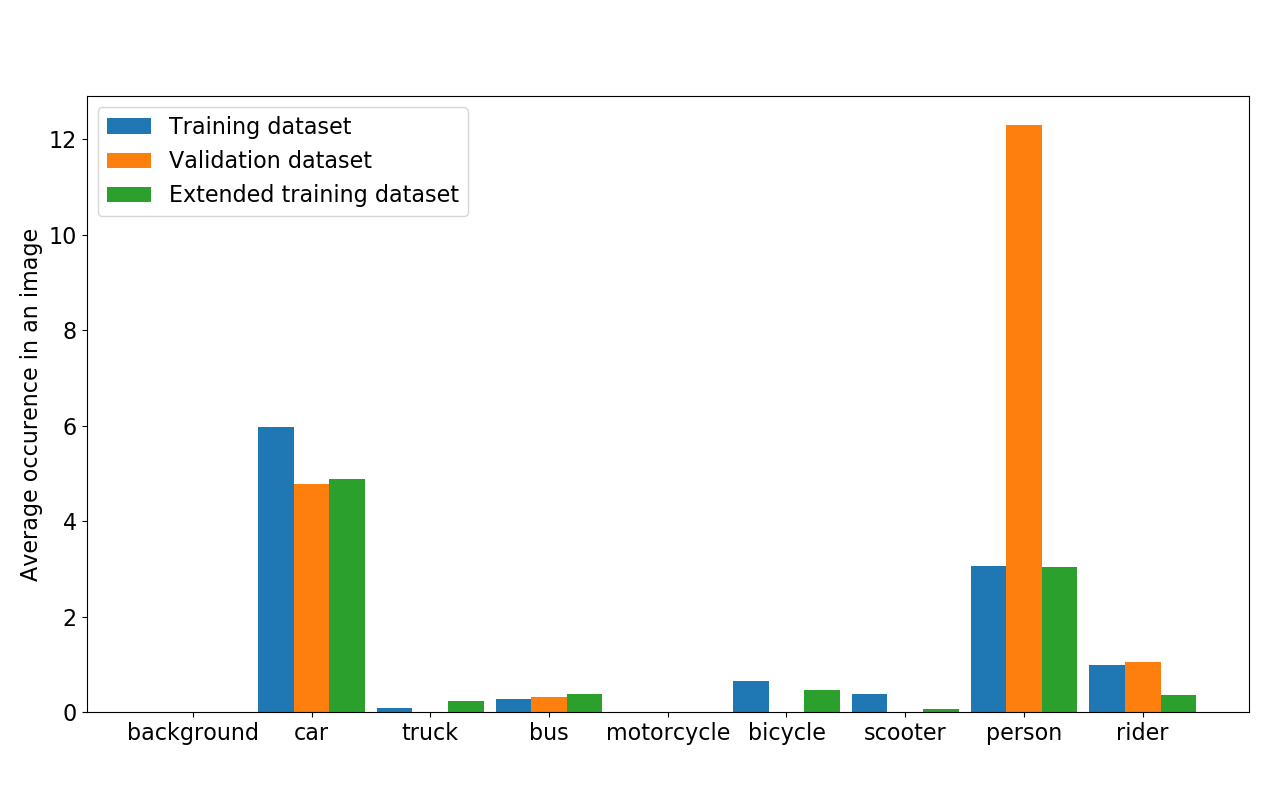
\includegraphics[width=0.49\textwidth]{label_distribution/comparison/avg_occ_comparison.png}} 
    \subfigure[]{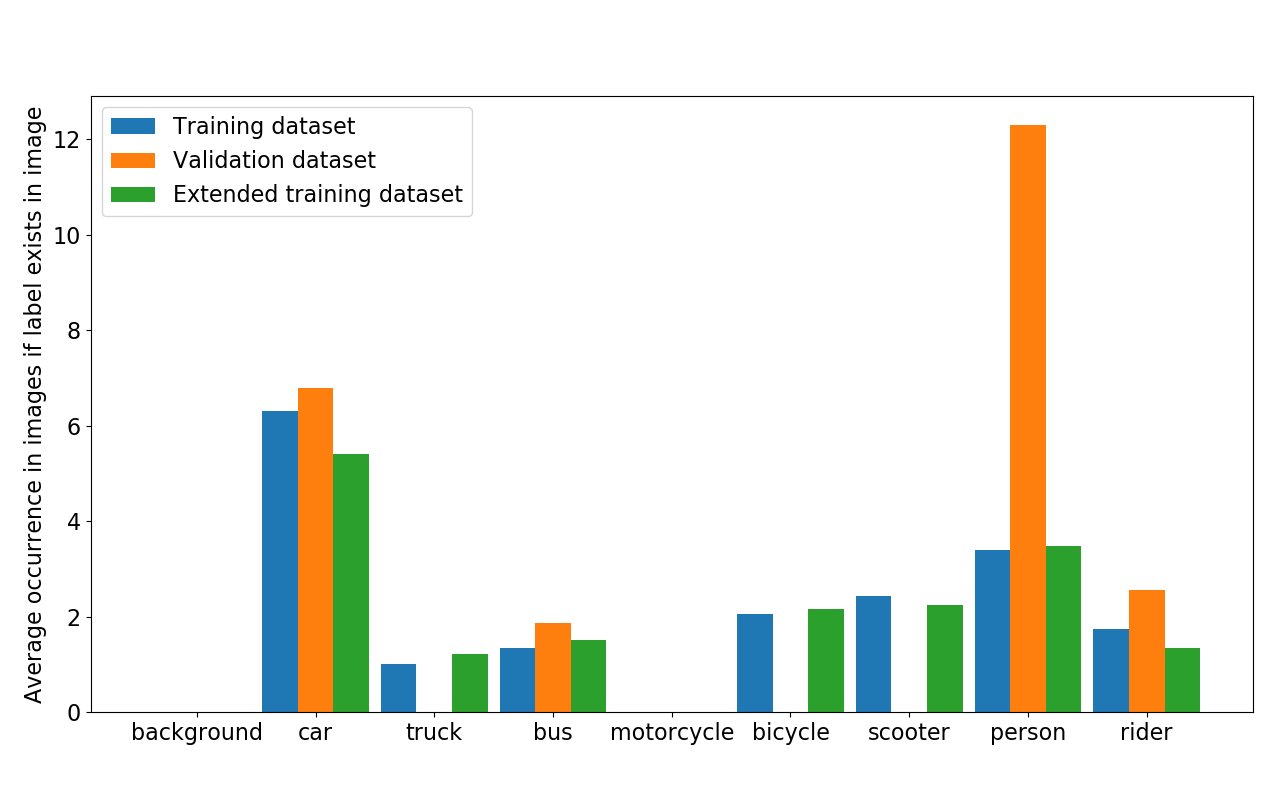
\includegraphics[width=0.49\textwidth]{label_distribution/comparison/avg_occ_if_label_exist_comparison.png}} 
    \caption{Average occurrence of labels (a) over all images (b) in images where the respective label exists.}
    \label{fig:occurrence}
\end{figure}

As a second part of the quantitative analysis, we performed a closer object exploration on the original training dataset and the validation set. This includes the mean area of bounding boxes for each object class as well as histograms of the ratio and size of the bounding boxes over all object classes, which are shown in Figure \ref{fig:objects_expl}. From Figure \ref{fig:objects_expl} (a), it can be seen that trucks and busses have the largest bounding boxes on average, which is consistent with our expectations. Additionally, Figure \ref{fig:objects_expl} (b) shows that there is an overall higher number of smaller bounding boxes in both the training and validation set. The similar distribution allows for the expectation of good validation performance, which shall be examined in the course of this report. Figure \ref{fig:objects_expl} (c) on the other hand shows the frequency of ratios of bounding boxes over both sets. Here, a high number of small ratios, i.e., close to quadratic bounding boxes, can be observed. After a sharp drop, a smaller number of objects has rectangular bounding boxes with a higher ratio of height and width. This leads to the conclusion that there are either somewhat quadratic or somewhat slim bounding boxes, but no continuous transition between the two in both the original training set and the validation set.

Furthermore, \ref{fig:objects_expl} (d) and (e) give the height and width of all bounding boxed for the original training and the validation set as clusters, respectively. Similarly as above, the different distribution of bounding box ratio and size in the original training set and the validation set can be observed. As we have observed from Figure \ref{fig:occurrence}, there is a higher number of persons annotated in the validation set. This is consistent with Figure \ref{fig:objects_expl}, where the bounding boxed for persons, which are small in width but large in height, can be observed distinctly in the cluster. Note that subplots (d) and (e) in Figure \ref{fig:objects_expl} are scaled differently for better visibility. There are however larger bounding boxes in the training set compared to the validation set (consistent with the right tail of subplot (b) of Figure \ref{fig:objects_expl}). As an hypothesis, this could be due to the absence of trucks and busses in the validation set, which are the two largest objects if compared at the same distance. Additionally, there is a high number of cars in the training set, which, if in traffic and captured from a close distance, also have large bounding boxes.

\begin{figure}[t!]
    \centering
    \subfigure[]{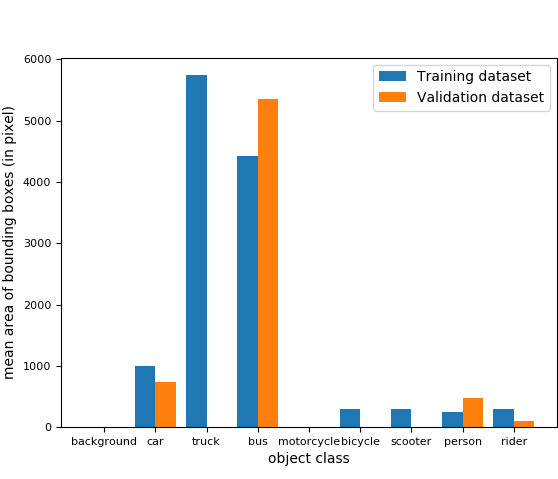
\includegraphics[width=0.32\textwidth]{object_exploration/mean_area_cropped.png}}
    \subfigure[]{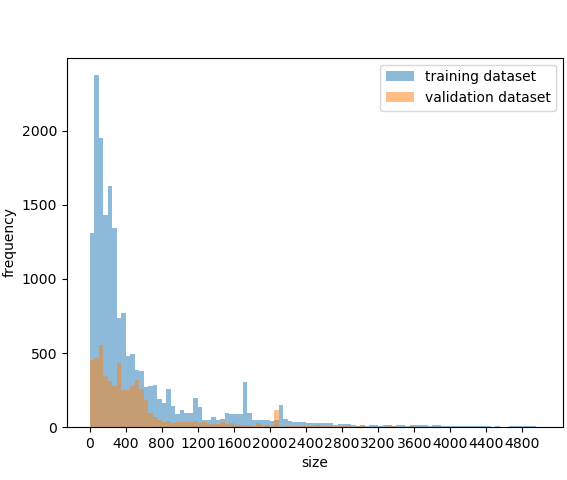
\includegraphics[width=0.32\textwidth]{object_exploration/sizes_cropped.png}}
    \subfigure[]{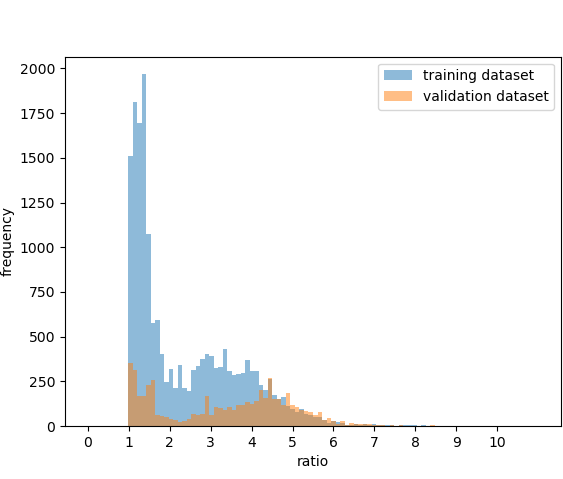
\includegraphics[width=0.32\textwidth]{object_exploration/ratios_cropped.png}}
    \subfigure[]{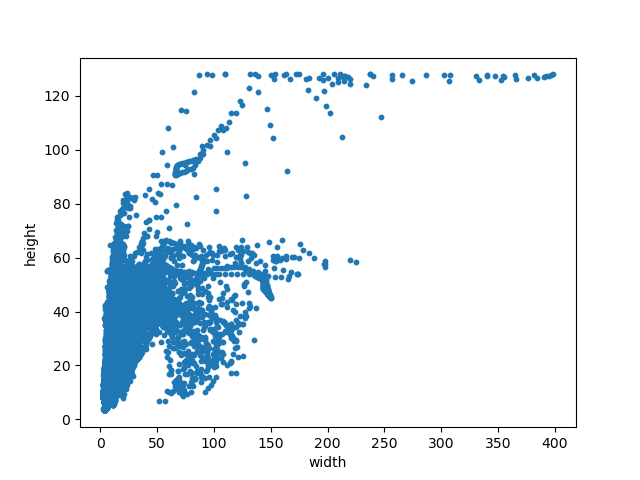
\includegraphics[width=0.4\textwidth]{object_exploration/wh_cluster_train.png}}
    \subfigure[]{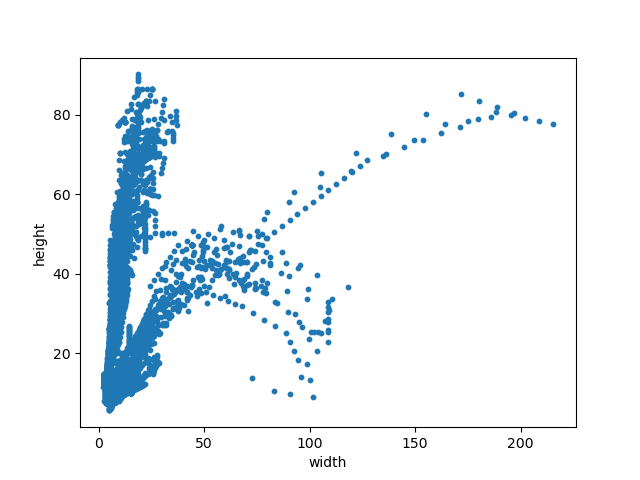
\includegraphics[width=0.4\textwidth]{object_exploration/wh_cluster_val.png}}
    \caption{(a) Mean area of bounding boxes (in pixels) for respective object class (b) histogram of all bounding box sizes (c) histogram of all bounding box ratios (d) cluster of bounding box height and width in the original training set and (e) in the validation set.}
    \label{fig:objects_expl}
\end{figure}

Finally, we investigated some border cases in the dataset to complement the mean observations. Figure \ref{fig:extreme_train} shows the image from the original training set with the maximum (a) and minimum (b) number of annotated objects, the object with the maximum (c) and minimum (d) bounding box ratio and maximum (e) and minimum (f) bounding box size, and the images with the maximum number of cars (g) and persons (h), which are the two most prevalent object categories (see Figure \ref{fig:occurrence}). Figure \ref{fig:extreme_val} presents the same cases for the validation set. Interestingly, the maximum number of objects in an image in the original training set (subplot \ref{fig:extreme_train} (a)) is lower than our expectations, at a total of 22. Contrary to that, the validation set contains an image with 54 annotated objects, all of which are persons. Based on the training data, which only has an image with a maximum number of 9 persons, we expect this to be a challenging validation scenario for the model. Another notable case is subplot \ref{fig:extreme_val} (b), which shows the minimum number of annotated objects in the validation set, which is 4. However, there are a number of unannotated scooters in the middle of the image. The same is true for image \ref{fig:extreme_val} (c) as well as image \ref{fig:extreme_train} (b). Such missing annotations are fatal for the performance in the model if they occur in the training set \cite{xu2019missing} and entail an incorrect accuracy if they appear in the validation set. We have found further images with unannotated objects, among them bikes, busses, and cars, in the original training set, which we show in our video delivered alongside this report (slides {\color{red}{a-b}}). We will follow up on these observations in the following qualitative analysis of the data exploration.

\newpage
\begin{figure}[h!]
    \centering
    \subfigure[]{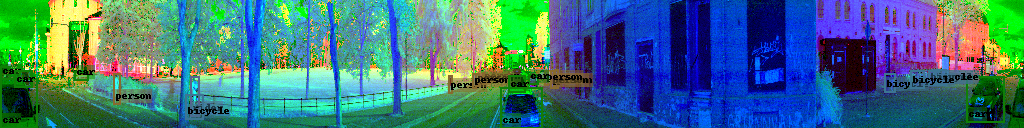
\includegraphics[width=\textwidth]{extreme_cases/train/maximum_num_objects.png}}
    \vspace{-0.15cm}
    \subfigure[]{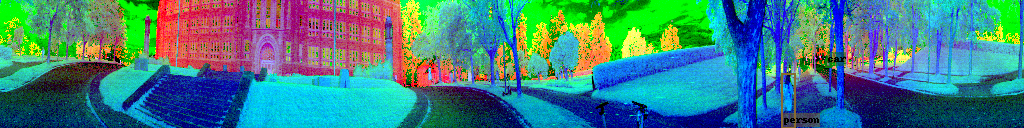
\includegraphics[width=\textwidth]{extreme_cases/train/minimum_num_objects.png}}
    \vspace{-0.15cm}
    \subfigure[]{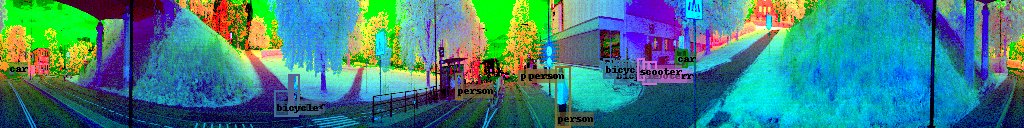
\includegraphics[width=\textwidth]{extreme_cases/train/maximum_ratio.png}}
    \vspace{-0.15cm}
    \subfigure[]{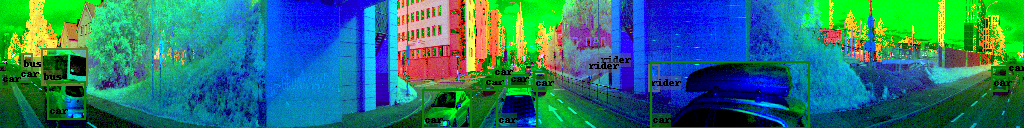
\includegraphics[width=\textwidth]{extreme_cases/train/minimum_ratio.png}}
    \vspace{-0.15cm}
    \subfigure[]{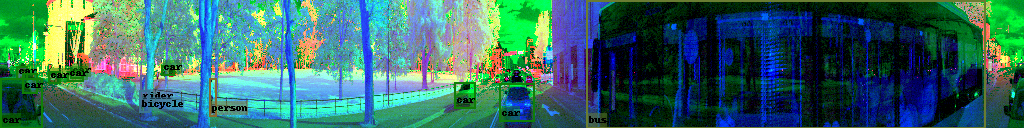
\includegraphics[width=\textwidth]{extreme_cases/train/maximum_size.png}}
    \vspace{-0.15cm}
    \subfigure[]{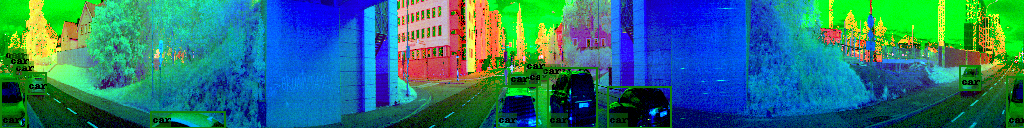
\includegraphics[width=\textwidth]{extreme_cases/train/minimum_size.png}}
    \vspace{-0.15cm}
    \subfigure[]{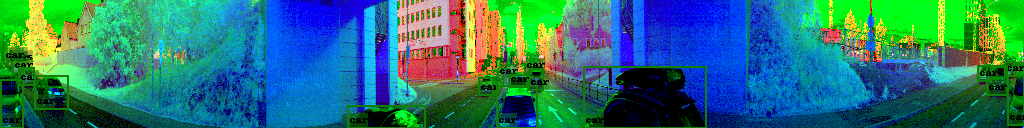
\includegraphics[width=\textwidth]{extreme_cases/train/maximum_num_cars.png}}
    \vspace{-0.1cm}
    \subfigure[]{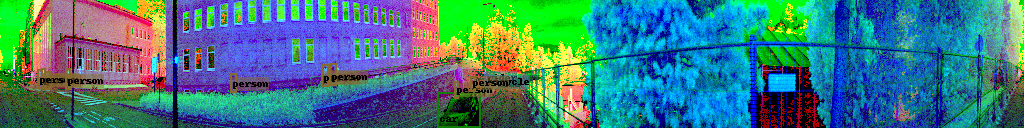
\includegraphics[width=\textwidth]{extreme_cases/train/maximum_num_persons.png}}
    \vspace{-0.49cm}
    \caption{The image from the original training set with (a) the maximum number of annotated objects (22) (b) the minimum number of annotated objects (2) (c) the object with the maximum bounding box ratio (51,046.40 pixels) (d) the object with the minimum bounding box ratio (9.99 pixels) (e) the object with the maximum bounding box size (11.15) (f) the object with the minimum bounding box ratio (1) (g) the maximum number of cars (18) (h) the maximum number of persons (9).}
    \label{fig:extreme_train}
\end{figure}
\newpage

\newpage
\begin{figure}[h!]
    \subfigure[]{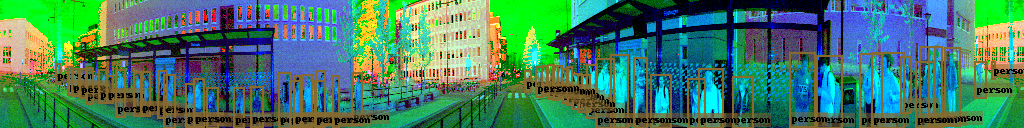
\includegraphics[width=\textwidth]{extreme_cases/val/maximum_num_objects.png}}
    \vspace{-0.15cm}
    \subfigure[]{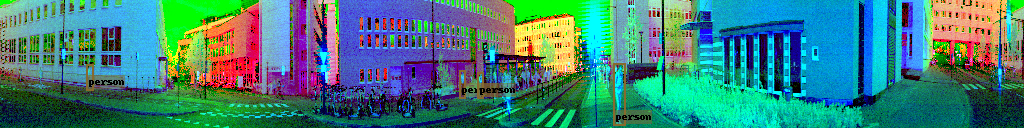
\includegraphics[width=\textwidth]{extreme_cases/val/minimum_num_objects.png}}
    \vspace{-0.15cm}
    \subfigure[]{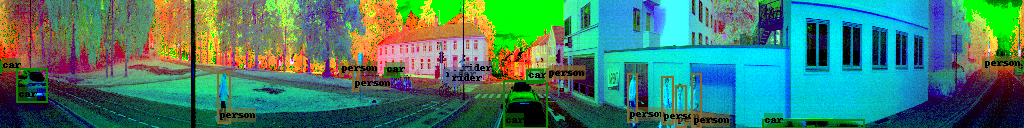
\includegraphics[width=\textwidth]{extreme_cases/val/maximum_ratio.png}}
    \vspace{-0.15cm}
    \subfigure[]{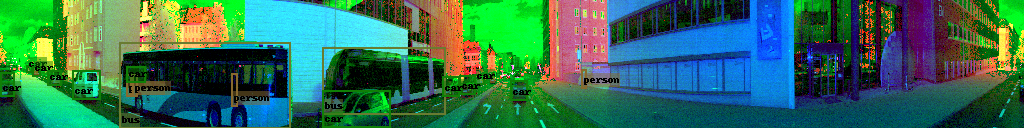
\includegraphics[width=\textwidth]{extreme_cases/val/minimum_ratio.png}}
    \vspace{-0.15cm}
    \subfigure[]{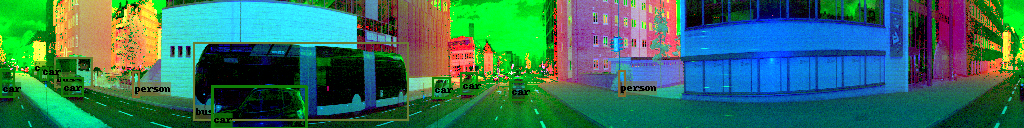
\includegraphics[width=\textwidth]{extreme_cases/val/maximum_size.png}}
    \vspace{-0.15cm}
    \subfigure[]{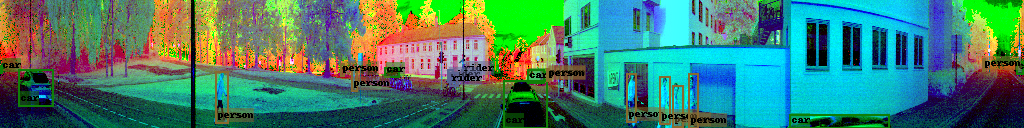
\includegraphics[width=\textwidth]{extreme_cases/val/minimum_size.png}}
    \vspace{-0.15cm}
    \subfigure[]{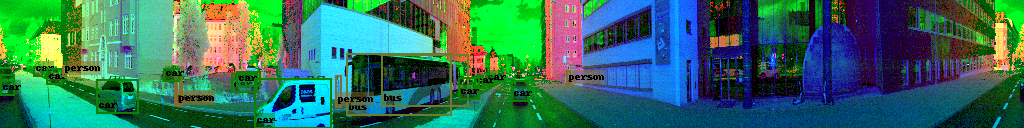
\includegraphics[width=\textwidth]{extreme_cases/val/maximum_num_cars.png}}
    \vspace{-0.1cm}
    \subfigure[]{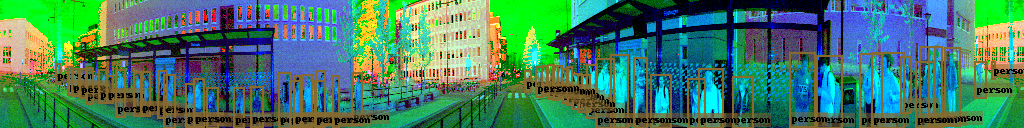
\includegraphics[width=\textwidth]{extreme_cases/val/maximum_num_persons.png}}
    \vspace{-0.49cm}
    \caption{The image from the validation set with (a) the maximum number of annotated objects (54) (b) the minimum number of annotated objects (4) (c) the object with the maximum bounding box ratio (16,760.03 pixels) (d) the object with the minimum bounding box ratio (19.17 pixels) (e) the object with the maximum bounding box size (11.43) (f) the object with the minimum bounding box size (1) (g) the maximum number of cars (12) (h) the maximum number of persons (54).}
    \label{fig:extreme_val}
\end{figure}
\newpage

\subsubsection*{Qualitative analysis}

Going more into depth into the content of the dataset, we oriented to the proposed approach in \cite{Karpathy2019} with the aim of estimating predictions and errors of the model and their reasons. A first questions to be evaluated on the basis of the explored data is whether local or global features are more significant to the outcome of the model performance. In our case, local features in the form of different vehicles and persons in traffic are the most important, while global features such as the brightness, weather or number of vehicles in traffic are of lesser importance. However, of the traffic participants, their global features should be learned by the model in order to classify the desired objects correctly, rather than differentiating within a class based on local features such as the colour of a person's jacket. Additionally, the global context of the objects needs to be correctly recognised by the model, such as the differentiation between a person riding a vehicle, thereby becoming a rider, and a pedestrian. This is a distinction we recognise as challenging, and expect the model to make mistakes in this regard.

The variation in the images is generally speaking low. The weather conditions in all captured images are consistent, where there is no precipitation, but snow on the side of the road in the majority of images. The winter conditions also entail that all pedestrians wear similar, winter-appropriate clothing, and that there are no convertibles and no motorcycles (see also Figure \ref{fig:occurrence}). In addition, all data is captured in a tightly limited local area of only a few kilometers within the same city. The volume of traffic is consistently low compared to other areas in the world, for example highways in the US or India.

The consistency of the labels in both the training and validation set is critically compromised however. As detailed above and in the video delivered alongside this report, a significant number of labels is either missing or incorrect. In addition to the problems already discussed above, this also leads to further inconsistencies such as the number of riders compared to the number of vehicles that can transport riders. Therefore, further preprocessing in the form of quality-checking the annotations would be appropriate and expected to improve the model performance across different approaches.

The level of detail in terms of resolution in the evaluated dataset is low. On the one hand, this enables somewhat reasonably efficient training, as the size of the data is limited. On the other hand, the objects to be classified are in many cases hard to detect and correctly bound even for humans, as we experienced during the annotation task of this project at first hand. Therefore, further downsampling of the images is not an option.

As a last point of observation, we conclude that the spatial position of objects in the images matters in the classification task at hand, and should not be average-pooled out. In the context of autonomous driving, which the dataset at hand is arguably relevant for, vehicles and persons should be recognised in any area of the image, as the capturing sensor could for example be looking down onto or up towards a scene of traffic due to hilly roads.

\section*{Task 2: Model Creation}

\subsection*{Task 2.1: Baseline Model}

\begin{table}[t!]
    \small
    \centering
    \begin{tabular}{l|l|c|c|c|c}
        \hline
         Is Output & Layer Type & Number filters & Kernel size & Stride & Padding  \\
         \hline
         & Conv2D & 32 & 3 & 1 & 1 \\
         & ReLU & & & & \\
         & MaxPool2D & & 2 & 2 & 0\\
         & Conv2D & 64 & 3 & 1 & 1\\
         & ReLU & & & & \\
         & Conv2D & 64 & 2 & 1 & 0 \\
         & ReLU & & & &  \\
         & Conv2D & 128 & 2 & 2 & 1\\
         Yes - resolution: $32\times 256$ & ReLU & & & & \\
         \hline
         & ReLU & & & &\\
         & Conv2D & 128 & 3 & 1 & 1\\
         & ReLU & & & & \\
         & Conv2D & 256 & 3 & 2 & 1\\
         Yes - resolution: $16\times 128$ & ReLU & & & & \\
         \hline
         & Conv2D & 256 & 3 & 1 & 1\\
         & ReLU & & & & \\
         & Conv2D & 128 & 3 & 2 & 1\\
         Yes - resolution: $8\times 64$ & ReLU & & & & \\
         \hline
         & ReLU & & & & \\
         & Conv2D & 128 & 3 & 1 & 1\\
         & ReLU & & & & \\
         & Conv2D & 128 & 3 & 2 & 1\\
         Yes - resolution: $4\times 32$ & ReLU & & & & \\
         \hline
         & ReLU & & & & \\
         & Conv2D & 128 & 3 & 1 & 1\\
         & ReLU & & & & \\
         & Conv2D & 64 & 3  & 2 & 1\\
         Yes - resolution: $2\times 16$ & ReLU & & &  & \\
         \hline
         & ReLU & & & & \\
         & Conv2D & 128 & 2 & 2 & 1\\
         & ReLU & & & & \\
         & Conv2D & 64 & 2 & 1 & 0\\
         Yes - resolution: $1\times 8$ & ReLU & & & &\\
         \hline
    \end{tabular}
    \caption{Architecture of baseline model from Task 2.1.}
    \label{tab:baseline}
\end{table}
For this task, we followed all changes given in the task description. The resulting architecture of our baseline model is summarized in Table \ref{tab:baseline}. As recommended, the second max-pool layer of the orginal SSD architecture of assignment 4  was removed and the kernel size of the last two convolutions was set to 2. The baseline model can be found in the configuration file \texttt{configs/tdt4265\_task2-1.py}. It has a total number of 2,750,240 parameters.

The best\footnote{In all quantitative analyses, we give the best mAP@0.5:0.95 that we recorded during the number of epochs trained, which is not always obtained in the last epoch. We implemented this by always saving the current best model.} mAP@0.5:0.95 for the baseline model is 0.037 after 30 epochs, 0.046 after 50 epochs, and 0.054 after 125 epochs. The inference speed is 14.32 frames per second with a total runtime of approximately 6.98 seconds. Plots of the total loss, classification loss, regression loss and mAP can be found in Figure \ref{fig:loss-2-1}. Additionally, we decided to show the AP plots for object classes car and person, which are the two prevalent classes. It can be clearly observed that the AP for cars improves faster and more steadily than for persons, giving a first indication that the classification of the latter is a harder problem for the model. Additionally, we can observe that the AP for class car improves very similarly with the mAP. Knowing that car is the prevalent class in the training set, we can therefore conclude that the training in the baseline model is dominated by this class, and does not perform as well on the less prevalent classes. This can again be seen when observing the AP for the class person in Figure \ref{fig:loss-2-1} (f).

\begin{figure}[t!]
    \centering
    \subfigure[]{\includesvg[width=0.32\textwidth]{Task2-1/loss_total_loss.svg}}
    \vspace{-0.15cm}
    \subfigure[]{\includesvg[width=0.32\textwidth]{Task2-1/loss_classification_loss.svg}}
    \subfigure[]{\includesvg[width=0.32\textwidth]{Task2-1/loss_regression_loss.svg}}
    \subfigure[]{\includesvg[width=0.32\textwidth]{Task2-1/metrics_mAP.svg}}
    \subfigure[]{\includesvg[width=0.32\textwidth]{Task2-1/metrics_AP_car.svg}}
    \subfigure[]{\includesvg[width=0.32\textwidth]{Task2-1/metrics_AP_person.svg}}
    \vspace{-0.4cm}
    \caption{(a) Total loss (b) classification loss (c) regression loss (d) mAP (e) AP for class car (f) AP for class person for baseline model of Task 2.1 trained for 125 epochs.}
    \label{fig:loss-2-1}
\end{figure}


\subsection*{Task 2.2: Data Augmentation}
In terms of data augmentation, we experimented with six different transformations. In addition to the two already implemented, horizontal flip and random crop, we implemented augmentations through random Gaussian blur, random translation, random dropout and random noise. Visualisations of all six augmentations are shown in Figure \ref{fig:data_augment}, and details can be found in the config files \texttt{configs/tdt4265\_task2-2\_hori\_flip.py}, \texttt{[...]\_crop.py}, \texttt{[...]\_gaussian\_blur.py},\\ \texttt{[...]\_translation.py}, \texttt{[...]\_dropout.py} and \texttt{[...]\_noise.py}.


\begin{figure}[h!]
    \subfigure[]{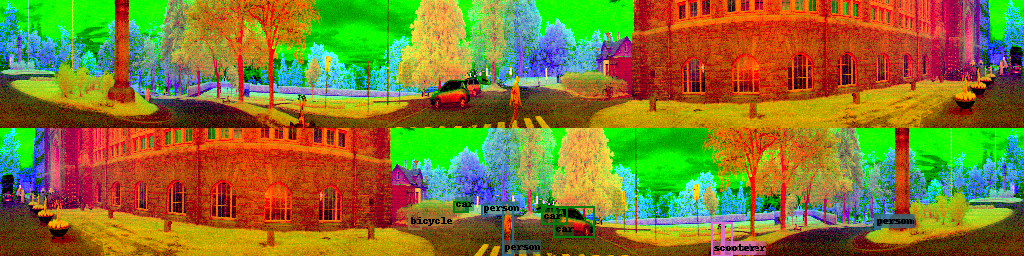
\includegraphics[width=0.49\textwidth]{Task2-2/horizontal_flip/image_9.png}}
    \vspace{-0.15cm}
    \subfigure[]{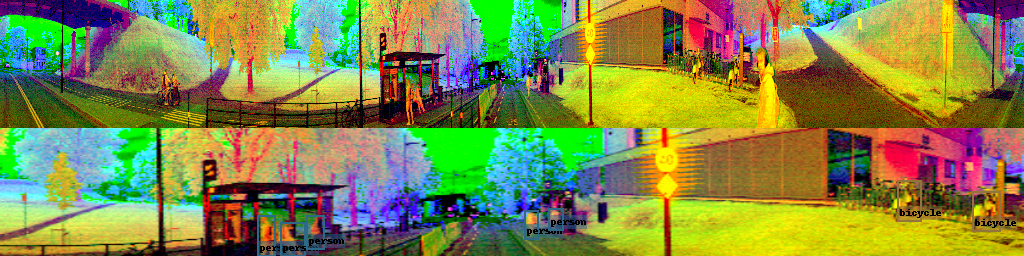
\includegraphics[width=0.49\textwidth]{Task2-2/crop/image_275.png}}
    \vspace{-0.15cm}
    \subfigure[]{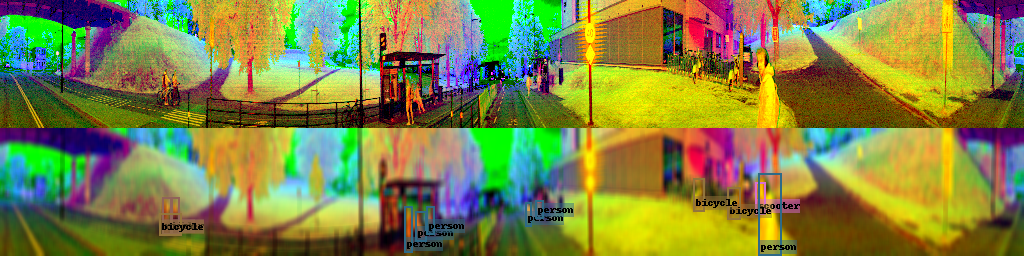
\includegraphics[width=0.49\textwidth]{Task2-2/gaussian_blur/image_275.png}}
    \vspace{-0.15cm}
    \subfigure[]{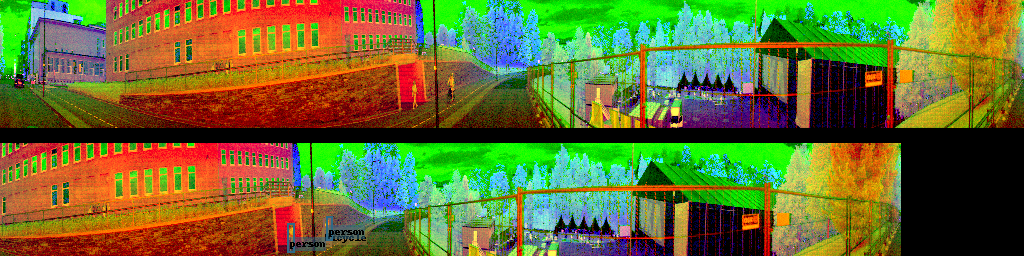
\includegraphics[width=0.49\textwidth]{Task2-2/translation/image_175.png}}
    \vspace{-0.15cm}
    \subfigure[]{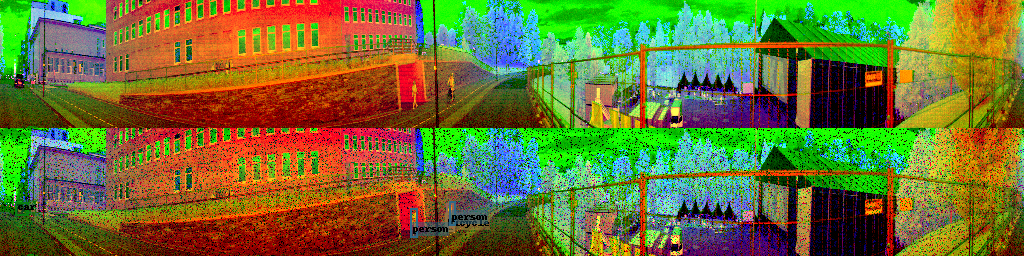
\includegraphics[width=0.49\textwidth]{Task2-2/dropout/image_175.png}}
    \vspace{-0.15cm}
    \hspace{0.2cm}\subfigure[]{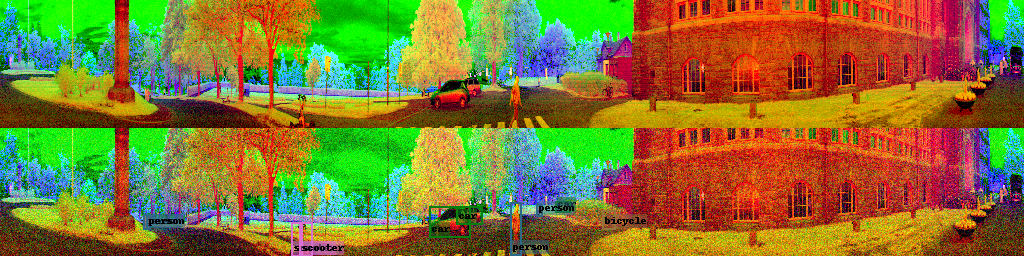
\includegraphics[width=0.49\textwidth]{Task2-2/noise/image_9.png}}
    \vspace{-0.15cm}
    \caption{Data augmentation by means of (a) random horizontal flip (b) random crop (c) random Gaussian blur (d) random translation (e) random dropout (f) random noise. The top image of each subplot is the original image, the bottom image the augmented image.}
    \label{fig:data_augment}
\end{figure}

\subsubsection*{Quantitative Analysis}
Plots of losses for the baseline model in combination with the different augmentations are shown in Figure \ref{fig:loss-2-2-better}, which shows all augmentation approaches that improve the performance compared to the baseline system, and Figure \ref{fig:loss-2-2-worse}, showing all approaches with worse performance. Overall, each augmentation is evaluated individually with the baseline model, i.e., augmentations are not stacked upon each other. The best mAP@0.5:0.95 after 125 epochs is 0.057 with random horizontal flip, 0.062 with random crop, 0.059 with random Gaussian blur, 0.062 with random translation, 0.055 with random dropout and 0.050 with random noise.

Despite training for an increased number of epochs, none of the data augmentation methods improve the mAP significantly compared to the baseline model of Task 2.1. The best empirical argument can be made for random translation and random crop, which both achieve the highest mAP, and arguably provide similar transformations on the training data. This observation supports our assumption that learning objects independent of their spatial position is important to the performance of the model. Furthermore, with the translation of the image, the model learns features of categories with less context, since for example the pavement under a person could be shifted out of the image. While the training dataset provides this, the augmentation by cropping and translating adds to the model experiencing such situations. Contrary to that, adding noise or dropping out pixels are not helpful to the model. We presume that the resolution of the images is already a lower bound for the model, and adding further disturbance to the information presented is too much of a challenge. Horizontal flip and Gaussian blur barely change the performance of the model.

The inference speed and the number of parameters do not change under data augmentation.

\begin{figure}[t!]
    \centering
    \subfigure[]{\includesvg[width=0.32\textwidth]{Task2-2/better/loss_total_loss4.svg}}
    \vspace{-0.15cm}
    \subfigure[]{\includesvg[width=0.32\textwidth]{Task2-2/better/loss_classification_loss4.svg}}
    \subfigure[]{\includesvg[width=0.32\textwidth]{Task2-2/better/loss_regression_loss4.svg}}
    \subfigure[]{\includesvg[width=0.32\textwidth]{Task2-2/better/metrics_mAP4.svg}}
    \subfigure[]{\includesvg[width=0.32\textwidth]{Task2-2/better/metrics_mAP@0.5_4.svg}}
    \subfigure[]{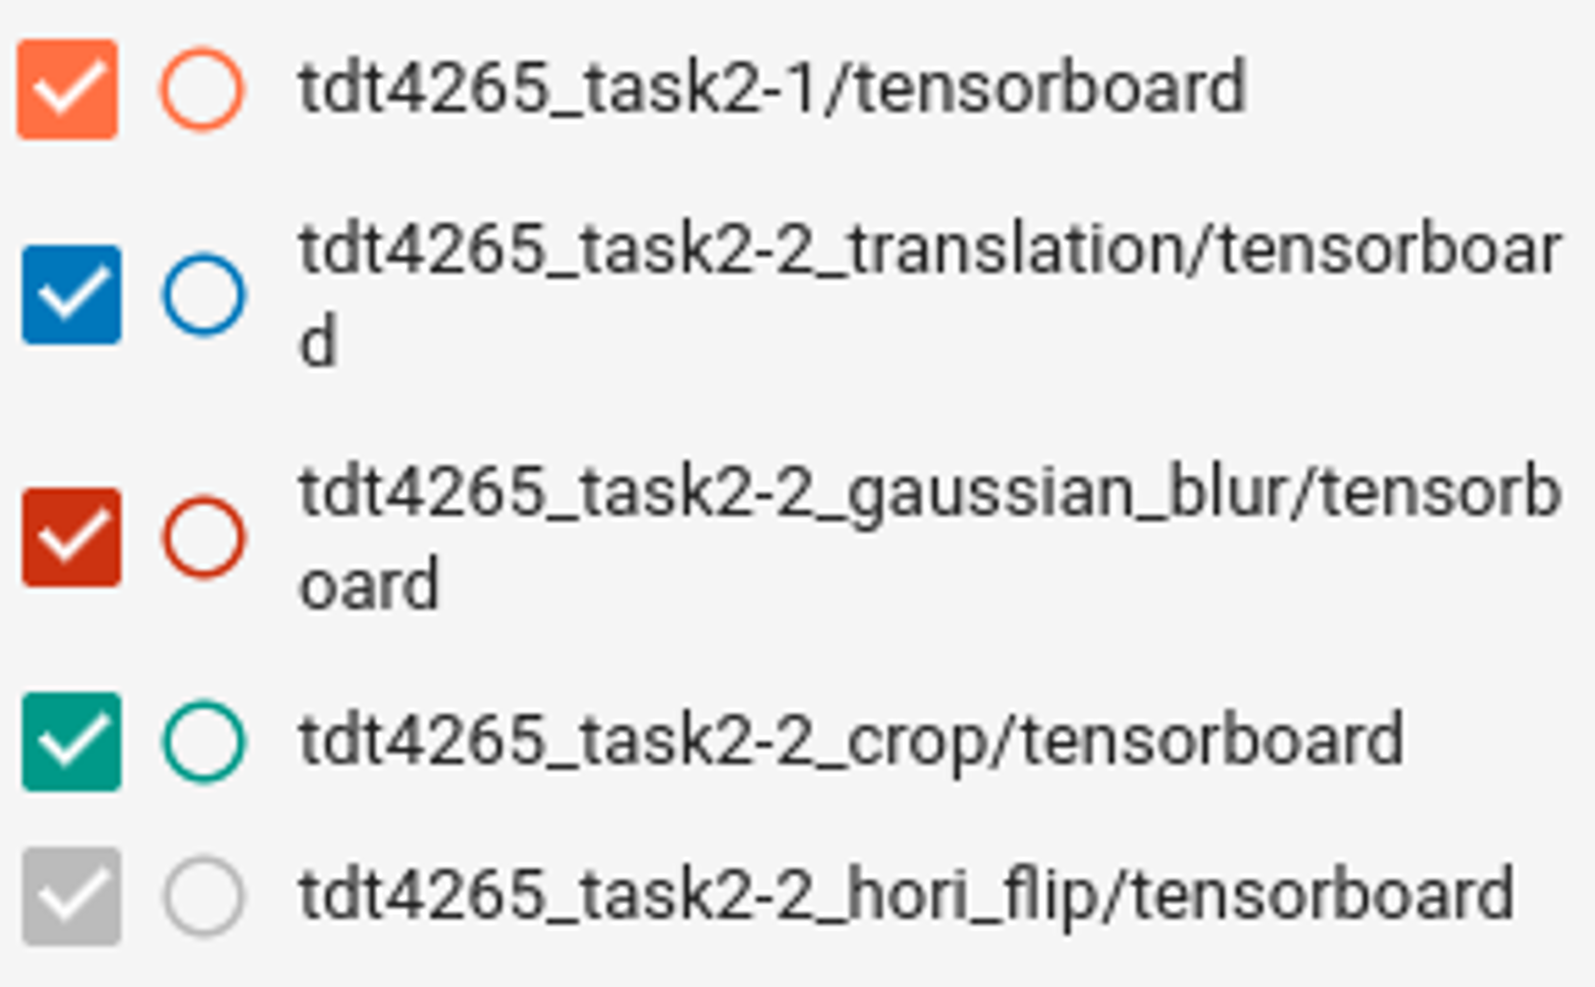
\includegraphics[width=0.32\textwidth]{Task2-2/legend-2-2-better1.png}}
    \vspace{-0.3cm}
    \caption{(a) Total loss (b) classification loss (c) regression loss (d) mAP (e) mAP@0.5 (f) legend for data augmentation of Task 2.2 trained for 125 epochs, performing better than the baseline model from Task 2.1 (in terms of mAP).}
    \label{fig:loss-2-2-better}
\end{figure}

\begin{figure}[t!]
    \centering
    \subfigure[]{\includesvg[width=0.32\textwidth]{Task2-2/worse/loss_total_loss2.svg}}
    \vspace{-0.15cm}
    \subfigure[]{\includesvg[width=0.32\textwidth]{Task2-2/worse/loss_classification_loss2.svg}}
    \subfigure[]{\includesvg[width=0.32\textwidth]{Task2-2/worse/loss_regression_loss2.svg}}
    \subfigure[]{\includesvg[width=0.32\textwidth]{Task2-2/worse/metrics_mAP2.svg}}
    \subfigure[]{\includesvg[width=0.32\textwidth]{Task2-2/worse/metrics_mAP@0.5.svg}}
    \subfigure[]{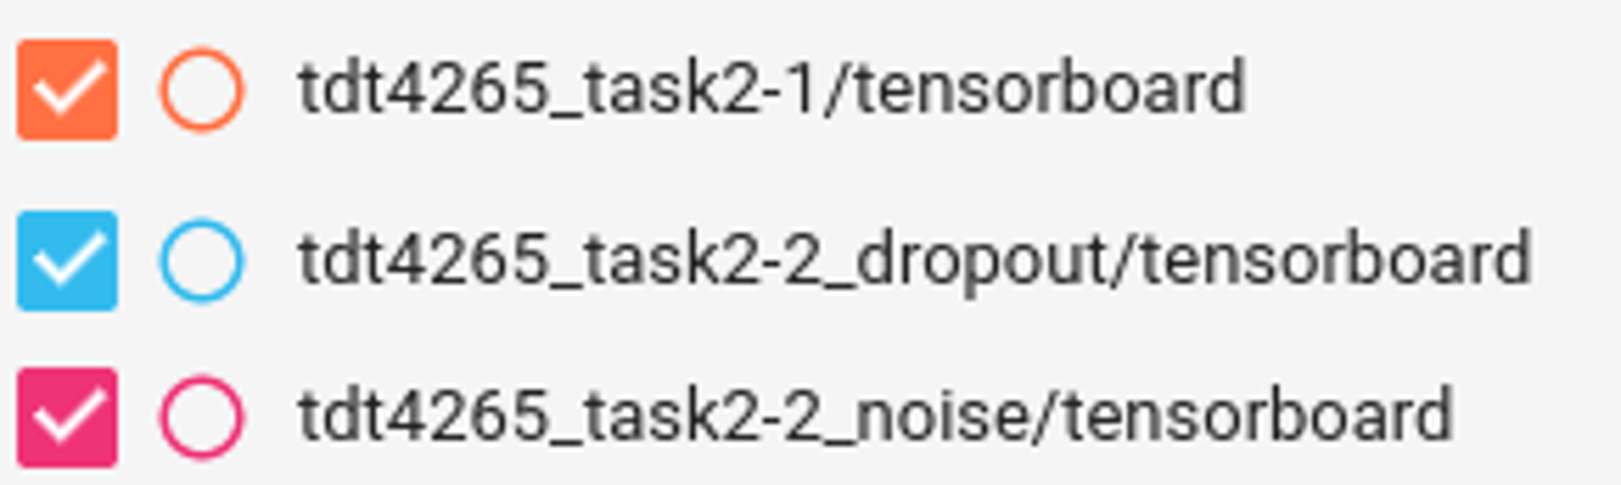
\includegraphics[width=0.32\textwidth]{Task2-2/legend-2-2-worse.png}}
    \vspace{-0.3cm}
    \caption{(a) Total loss (b) classification loss (c) regression loss (d) mAP (e) mAP@0.5 (f) legend for data augmentation of Task 2.2 trained for 125 epochs, performing worse than the baseline model from Task 2.1 (in terms of mAP).}
    \label{fig:loss-2-2-worse}
\end{figure}

\subsubsection*{Runtime Performance}
Loading the images from the original training set without any augmentations comes at a speed of approximately 104.83 images per seconds. In comparison, data loading with random crop achieves 120.73, random dropout 99.51, random blur 107.48, horizontal flip 101.15, random Gaussian noise 105.43, and finally random translation only 35.16 images per seconds, respectively.

\subsubsection*{Combining the Data Augmentation}
Finally, we combined the four data augmentations that yielded a better performance than the baseline model individually. A plot of the mAP using the combined augmentations can be found in Figure \ref{fig:data_augment_comparison} (a). The mAP@0.5:0.95 comes out at 0.54 after training for 167 epochs. While this does not give an improvement to the precision achieved with the Task 2.1 baseline model, its benefits will become evident once the model becomes more complex in Task 2.3.

The runtime for dataloading in this case dropped down to 48.82 images per second. Due to the high cost of data loading, and at the recommendation of one of the instructors, we decided to go forward with the following tasks without using data augmentation on the original training set. Only at the end of Task 2.3, we add the combined data augmentation back in (see Figure \ref{fig:data_augment_comparison} (b)) to evaluate its effect on the more complex model. 

\subsection*{Task 2.3: Implementing RetinaNet}

\subsubsection*{Feature Pyramid Network}
Coming from the Task 2.1 baseline mode, we replaced the first four layers of the model by the first four layers of the  pretrained ResNet34 model from the torchVision model zoo \cite{pytorchModelZoo}. For the fifth and sixth feature extraction layer, we used a sequence of a convolutional layer with 512 channels, kernel size 3, stride 1, padding 1 followed by ReLU activation function, a MaxPool2D layer with kernel size 2 and stride 2, a second convolutional layer with 256 channels, kernel size 3, stride 1 and padding 1, and a ReLU activation to conclude the feature extraction layer, respectively. Finally, we built the Feature Pyramid Network (FPN) on top of the six feature extraction layers as described in \cite{lin2017feature} with channel size 256 and the same number of aspect ratios for each layer, as anticipation for later use of deeper classification and regression heads and for better comparability and a more meaningful analysis.

Replacing the backbone of the baseline model with a FPN yielded a best mAP@0.5:0.95 after 100 epochs of 0.056. Details can be found in the config file \texttt{configs/tdt4265\_task2-3\_fpn}.  The implementation of the FPN can be found in the file \texttt{modeling/backbones/resnet34\_fpn.py}.  A plot of losses is given in Figure \ref{fig:loss-2-3}, where the FPN model is shown in dark blue. The model has a total number of 35,382,204 parameters and an inference speed of approximately 8.34 frames per seconds, with a total runtime of 11.10 seconds, which is faster than the Task 2.1 baseline model.

Applying the Resnet34 with a FPN on top only helps in detecting more medium sized objects. The detection of both large and small objects is not improved. This is a surprising result, since the objective of the FPN is mainly to provide semantically rich feature maps for smaller object sizes. Nevertheless, the mAP@0.5:0.95 increases by 0.2\% with 20 epochs less training time.

\textcolor{red}{Write about that FPN is supposed to help with the detection of smaller objects. mAP large decreases, mAP medium improves significantly, mAP small does not improve (yet).}

\textcolor{red}{To Do: Find out what small, medium, large means}

\subsubsection*{Focal Loss}
As described in the task, we replaced the loss function with Focal loss \cite{lin2017focal} with the recommendations made in the task description. This includes implementing Focal loss on top of the softmax cross-entropy loss, for which we added one-hot encoding of the given target labels. Details can be found in the file \texttt{ssd/modeling/focal\_loss.py}. For this task, we chose $\gamma = 2$ as recommended in \cite{lin2017focal} and set $\alpha = 0.1$ for the background class as indicated in the task. 

By these changes, the performance of best mAP@0.5:0.95 at 0.056 after 100 epochs is maintained in comparison to the FPN without Focal loss. The config file is \texttt{configs/tdt4265\_task2-3\_focal}. A plot of losses is given in Figure \ref{fig:loss-2-3}, where the model with Focal loss is shown in light blue. The inference speed and the total number of parameters remain the same as in the previous step.

\textcolor{red}{Talk about effect of Focal loss, expected/unexpected outcomes and reasons for them}


\subsubsection*{Deeper Classification and Regression Output Heads}
 We implemented deeper regression and classification heads following the architecture used in \cite{lin2017focal}. Details can be found in the file \texttt{ssd/modeling/RetinaDeep.py}. In our implementation, all feature map extractions share the same parameters, and in both heads, we used four convolutional layers with channel size 256, kernel size 3, stride 1 and padding 1 followed by ReLU activation each. The last layer of the classification head is now a convolutional layer with channel size n\_boxes $\times$ num\_classes, and the last layer of the regression head is a convolutional layer with channel size n\_boxes $\times$ 4.
 
Replacing the single-layer regression and classification output heads with deeper convolutional nets comes with an observable improvement in performance, with the best mAP@0.5:0.95 with in 100 epochs being 0.070. The config file is \texttt{configs/tdt4265\_task2-3\_heads}. The model has a total number of 39,203,894 parameters and an inference speed of 3.03 frames per second, for a total of 33.03 seconds. A plot of losses is given in Figure \ref{fig:loss-2-3}, where the model with deeper classification output heads is shown in orange.

\textcolor{red}{To Do: Argue about reason for performance improvement, better recognition for smaller objects, etc.}

\subsubsection*{Initialisation of Bias}

Technical changes:
\begin{itemize}
    \item initializing the weights and the bias as recommended in the paper \cite{lin2017focal}
    \item all bias parameter in both the regression and the classification head initialized to 0 despite the bias for the background class of the last layer of the classification head, which corresponds to the recommendation in the task
    \item all weights in both the regression and the classification head initialized to a gaussian distribution with mean of 0 and standard deviation of 0.1
\end{itemize}

\textcolor{red}{(Change this intro) Finally, initializing bias of last convolutional layer to the values described in the task description} gives a best mAP@0.5:0.95 of 0.069  after training for \textcolor{red}{100?} epochs. The config file is \texttt{configs/tdt4265\_task2-3\_init} \textcolor{red}{ + Refer to where in the code each component is implemented}. A plot of losses is given in Figure \ref{fig:loss-2-3}, where the model with improved initialization of the bias is shown in red.

\textcolor{red}{number of parameters, inference speed}

\begin{figure}[t!]
    \centering
    \subfigure[]{\includesvg[width=0.32\textwidth]{Task2-3/loss_total_loss3.svg}}
    \subfigure[]{\includesvg[width=0.32\textwidth]{Task2-3/loss_classification_loss3.svg}}
    \subfigure[]{\includesvg[width=0.32\textwidth]{Task2-3/loss_regression_loss3.svg}}
    \subfigure[]{\includesvg[width=0.32\textwidth]{Task2-3/metrics_mAP3.svg}}
    \subfigure[]{\includesvg[width=0.32\textwidth]{Task2-3/metrics_mAP@0.5_3.svg}}
    \subfigure[]{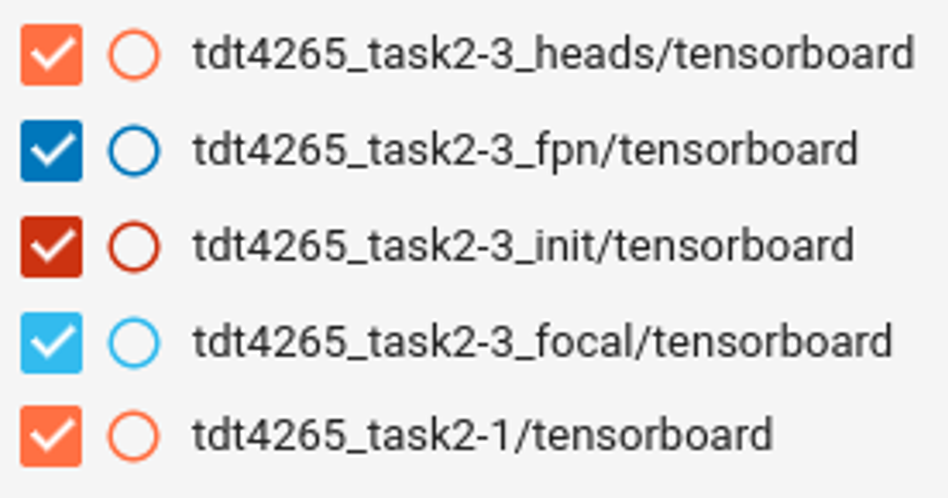
\includegraphics[width=0.32\textwidth]{Task2-3/legend-2-3.png}}
    \subfigure[]{\includesvg[width=0.32\textwidth]{Task2-3/metrics_mAP_small3.svg}}
    \subfigure[]{\includesvg[width=0.32\textwidth]{Task2-3/metrics_mAP_medium3.svg}}
    \subfigure[]{\includesvg[width=0.32\textwidth]{Task2-3/metrics_mAP_large3.svg}}
    \caption{(a) Total loss (b) classification loss (c) regression loss (d) mAP (e) mAP@0.5 (f) legend (g) mAP for small objects (h) mAP for medium objects (i) mAP for large objects for the iterations in Task 2.3 trained for 100 epochs. The baseline system of Task 2.1 is represented by the orange plot, which can be differentiated from the plot for the adapted regression heads as it was trained for a longer number of 125 epochs (and performs consistently worse).}
    \label{fig:loss-2-3}
\end{figure}

\subsubsection*{Adding Data Augmentation Back In}

\begin{figure}[]
    \centering
    \subfigure[]{\includesvg[width=0.32\textwidth]{Task2-2/final/metrics_mAP7.svg}}
    \subfigure[]{\includesvg[width=0.32\textwidth]{Task2-3/metrics_mAP_with_augmentations.svg}}
    \caption{\textcolor{red}{Add caption.}}
    \label{fig:data_augment_comparison}
\end{figure}

\textbf{\textcolor{red}{Analysis/discussion/comparison}}

\textcolor{red}{Final plot of inference speed as comparison? Same for number of parameters?}

\newpage
\subsection*{Task 2.4: Using the Exploration Knowledge}
\begin{itemize}
    \item Comprehensive technical description of the modifications introduced to the model in this task: short description of changes and reference to code/config files
    \item Quantitative analysis (?)
\end{itemize}

\subsection*{Task 2.5: Extending the Dataset}
Adapted focal loss $\alpha$ to distribution in extended training set as described for the original training set in Task 2.4? Same for anchor boxes?

\begin{itemize}
    \item Quantitative analysis on larger dataset
    \item Figure \ref{fig:loss-2-5}
    \item analyze the importance of a larger dataset
\end{itemize}

\begin{figure}[t!]
    \centering
    \subfigure[]{\includesvg[width=0.32\textwidth]{Task2-5/loss_total_loss5.svg}}
    \vspace{-0.15cm}
    \subfigure[]{\includesvg[width=0.32\textwidth]{Task2-5/loss_classification_loss5.svg}}
    \subfigure[]{\includesvg[width=0.32\textwidth]{Task2-5/loss_regression_loss5.svg}}
    \subfigure[]{\includesvg[width=0.32\textwidth]{Task2-5/metrics_mAP5.svg}}
    \subfigure[]{\includesvg[width=0.32\textwidth]{Task2-5/metrics_AP_car5.svg}}
    \subfigure[]{\includesvg[width=0.32\textwidth]{Task2-5/metrics_AP_person5.svg}}
    \vspace{-0.4cm}
    \caption{(a) Total loss (b) classification loss (c) regression loss (d) mAP (e) AP for class car (f) AP for class person for the Task 2.5 model trained on the original training set (orange) and the extended training set (grey) trained for 125 epochs.}
    \label{fig:loss-2-5}
\end{figure}



\section*{Task 3}

\subsection*{Task 3.1}
Delivered in Task 2 and 4.

\subsection*{Task 3.2}
Select three 3 of the most influential modeling decisions throughout the project and present a qualitative analysis. The qualitative analysis should highlight key aspects of your model and should be supported by qualitative
examples.

Example questions that your analysis and discussion can answer are:
\begin{itemize}
    \item What are the strengths of the model?
    \item What are the limitations of the model?
    \item What is the reason that a specific modeling decision improves metric X?
    \item Alternative methods to the modeling decision and why they are better/worse
\end{itemize}

We’ve included a set of scripts to help you to visualize predictions for your qualitative analysis. See the project
readme for more info

\textcolor{red}{Design decision: Model mit weniger Parametern maxpool instead of stride}

\subsection*{Task 3.3}
What are the weaknesses of the approach selected in the project if you were to deliver this to a customer?


\begin{itemize}
    \item Commonalities: The majority of images contain cars (and persons?)
    \item limitations: No motorcycle (due to snow), limited area captured, traffic in recorded area is rarely dense (compared to highways in the US, India, ...)
    \item Missing annotations are bad for performance
    \item Special value of dataset: Captured in one of the most northern parts of the world in winter conditions - evaluate network performance and autonomous driving under the impact of snow
    \item modelling decision derived from exploration:
        \begin{itemize}
            \item Spatial position matters (sensor is moving around landscape is hilly) - random crop for data augmentation meaningful, no average pooling
            \item (delete motorcycle class, as they are no motorcycles in the entire dataset?)
            \item Calibration of $\alpha$ value for focal loss based on label ratios
        \end{itemize}
\end{itemize}

\section*{Task 4}

As we are a group of two students, we chose two subtasks from Task 4: Task 4.1 and 4.2.

\subsection*{Task 4.1: Implementation BiFPN}
Choose two out of the four tasks

\subsection*{Task 4.2: Explaining the Model with CAM}
Class activation maps


\bibliographystyle{alpha}
\bibliography{sample}

\end{document}